\documentclass[reqno,11pt]{amsart}
\usepackage{amsmath, amsfonts, amsthm, amssymb, setspace, textcomp, enumerate, bbm, multirow, 
parskip, graphicx, pdfpages}
\usepackage{geometry}
%\usepackage[showframe]{geometry}
\geometry{hmargin={1in},vmargin={1in}}

\usepackage[hyphens]{url}
\usepackage{hyperref}
\hypersetup{breaklinks=true}

\pagestyle{plain}



\allowdisplaybreaks
\title{An analysis of US work stoppages and employee wages}

\author[N. Cornelius]{Nyssa Cornelius}
\email{nyssa.cornelius@du.edu}

\author[C. Jennings-Shaffer]{Chris  Jennings-Shaffer}
\email{christopher.jennings-shaffer@du.edu}


\begin{document}
\allowdisplaybreaks
\maketitle



\section{Introduction}

The GitHub repository for this project is located at
\url{https://github.com/NyssaCornelius/FProj}. The Binder link for this project
is \href{https://mybinder.org/v2/gh/NyssaCornelius/FProj/main}{Binder link}.
The main Jupyter Notebook for our project is FinalNotebook.ipynb. This file is available
on github and is also uploaded to the 2DU platform with this report.


The data sets are taken from the U.S. Bureau of Labor statistics (\url{https://www.bls.gov/}). 
For work stoppages, we used the excel file at \url{https://www.bls.gov/web/wkstp/monthly-listing.xlsx}.
This file contains information on each work stoppage in the US from 1993 on that involved at
least 1000 workers. Information about the columns is given in the following table
(all columns are stored as text).

\begin{tabular}{ccl}
column & basic type & description
\\\hline
Organizations involved 
	& 
	nominal
	&
	$\substack{\displaystyle\text{The company or branch of government where the}
	\\\displaystyle\text{work stoppage occurred.}}$
\\
States
	&
	nominal
	&
	The states where the work stoppage occurred.
\\
Areas
	&
	nominal
	&
	$\substack{\displaystyle\text{The geographic areas where the work stoppage }
	\\\displaystyle\text{occurred.}}$
\\
Ownership
	&
	nominal
	&
	$\substack{\displaystyle\text{This is either private industry (private sector) or}
	\\\displaystyle\text{state/local government (public sector).}}$
\\
Industry code	
	&
	numerical
	&
	$\substack{\displaystyle\text{The 2017 NAICS code describing the industry}
	\\\displaystyle\text{associated to the work stoppage.}}$
\\
Union	
	&
	nominal
	&
	$\substack{\displaystyle\text{The name of the union associated with the work} 
	\\\displaystyle\text{stoppage.}}$
\\
Union acronym	
	&
	nominal
	&
	The acronym for the union.
\\
Union Local	
	&
	nominal
	&
	$\substack{\displaystyle\text{A number or word description of the local union}
	\\\displaystyle\text{associated with the work stoppage.}}$
\\
Bargaining unit	
	&
	nominal
	&
	$\substack{\displaystyle\text{A description of the bargaining unit for}
	\\\displaystyle\text{the work stoppage (usually empty).}}$
\\
Work stoppage beginning date	
	&
	ordinal
	&
	Start date of the work stoppage.	
\\
Work stoppage ending date	
	&
	ordinal
	&
	End date of the work stoppage.	
\\	
Number of workers
	&
	numerical
	&
	$\substack{\displaystyle\text{The number of workers involved in the work}
	\\\displaystyle\text{stoppage.}}$
\\
$\substack{\displaystyle\text{Days idle cumulative}\\\displaystyle\text{for this work stoppage}}$
	&
	numerical
	&
	The total duration of the work stoppage.
\\
Note
	&
	nominal
	&
	$\substack{\displaystyle\text{Any notes about the work stoppage (e.g., the}
	\\\displaystyle\text{union changed names or the number of workers}
	\\\displaystyle\text{involved changed during the work stoppage).}}$
\end{tabular}


Employment statistics at the national level are taken from 
\url{https://download.bls.gov/pub/time.series/ce/},
specifically from 
\href{https://download.bls.gov/pub/time.series/ce/ce.industry}{ce.industry},
\href{https://download.bls.gov/pub/time.series/ce/ce.series}{ce.series},
and
\href{https://download.bls.gov/pub/time.series/ce/ce.data.0.AllCESSeries}{ce.data.0.AllCESSeries}
Since a full description of these data sets are given in 
\href{https://download.bls.gov/pub/time.series/ce/ce.txt}{ce.txt}, 
let us be a bit brief in the description. 
The file ce.series contains an entry for each type of data stored
at the national level (for example:
``Average hourly earnings of all employees, stone mining and quarrying, seasonally adjusted''),
whereas the actual data values for this are stored in 
ce.series; they are joined on the column series\_id (e.g., CES1021231003).
The file ce.series also contains a column for industry\_code, which is matched
to the description of the industry code in ce.industry. In ce.industry, there is
partial information to match an industry code of ce.series with an NAICS industry code of
work stoppage data. This is discussed in greater detail in Section 3.


Similarly, employment statistics at the state level are taken from 
\url{https://download.bls.gov/pub/time.series/sa/},
specifically
\href{https://download.bls.gov/pub/time.series/sa/sa.series}{sa.series},
\href{https://download.bls.gov/pub/time.series/sa/sa.data.0.Current}{sa.data.0.Current},
\href{https://download.bls.gov/pub/time.series/sa/sa.industry}{sa.industry},
and
\href{https://download.bls.gov/pub/time.series/sa/sa.state}{sa.state},
with a detailed description of the data sets given in
\href{https://download.bls.gov/pub/time.series/sa/sa.txt}{sa.txt}.
The file sa.series contains an entry for each type of data stored
at the state level and the actual data for the entries are stored in 
sa.data.0.Current, again joining on the column series\_id.
We use sa.state to decode the state for a series from numeric to string.
However, this time sa.industry does contain even partial information to 
match industry codes, but it does at least give an English description
of the codes. This is also discussed in greater detail in Section 3.



The minimum wage data set is an amalgamation of data pulled from two locations, 
the first being the original location of the data set: 
\href{https://www.dol.gov/agencies/whd/minimum-wage}{Department of Labor Minimum Wage Data}, 
the second being Kaggle: 
\href{https://www.kaggle.com/lislejoem/us-minimum-wage-by-state-from-1968-to-2017}{DOL Minimum Wage Data Scraped and Cleaned}. 
The original dataset, as observed with many of this project’s government datasets contains Unicode characters unrecognizable 
to various python packages rendering a scrape of the html table more labor intensive than the Kaggle dataset of the same information. 
The Kaggle dataset was a web scrape of the original U.S. Department of Labor table for historical minimum wages. 
This Kaggle dataset was further cleaned for clarity of nomenclature and parsimony of data. Extraneous columns such as 
Federal Minimum wage were removed as the Effective Minimum Wage and Wage in 2020 dollars were more informative. 
This is because when a state minimum wage is below the federal minimum wage for any given year, the effective minimum 
wage becomes the federal minimum wage. There were no states omitted from the data. The years of the data ranged from 
1968 to 2020. The Effective Minimum Wage in 2020 Dollars column was kept as a point of reference in the visualizations 
and the dataset so that a viewer of the data could more easily understand the value of the minimum wages at the time they were set.

The last dataset used for this project was the State-Metro Employment and Wage Data (hereby referred to as smdata), 
originally located 
\href{https://download.bls.gov/pub/time.series/sm/sm.data.1.AllData}{here}
within the U.S. Bureau of Labor Statistics site. This data was used in attempt to quantify average hourly wages by 
industry. Unfortunately, further on in the analysis portion of this project, it became evident that the individuals 
preparing the data were less than uniform in their choice, updating, and creation of the industry codes found between 
this and our other datasets. For example, the industry codes used in smdata were a combination of the 2012 NAICS Codes 
(other data used 2017 NAICS codes) and codes created by either the data preparers or someone within the organization. 
The NAICS codes, traditionally, no longer than 6 digits, are written so that 2 digits are the largest industry grouping, 
3 digits gets more granular in industry, and so on, until the 6-digit code, which is the highest level of specificity for 
industry. However, for reasons undisclosed in the dataset, the preparers added a 2-digit ``supersector'' code on to the 
original NAICS code classification, which oftentimes was redundant or overgeneralized two industry groupings into one. 
Again, the true reasonings for this are not present in the documentation for the dataset. Best attempts were made to make 
inferences from the overgeneralized groupings to the other datasets that did not have these ``supersector'' codes, but they
 are not a 1-to-1 comparison by any means. There are also some local government industries included in the smdata that 
 were not present in the 
\href{https://www.census.gov/naics/?58967?yearbck=2012}{2012 NAICS Codes} or 
\href{https://www.census.gov/naics/?58967?yearbck=2017}{2017 NAICS Codes}
 and thus were excluded. 




The choice of using these data sets is that they contained the greatest
amount of information we could locate. Upon reviewing the literature,
they are the standard sets to use (and have been for a long time).
To load in the data, we downloaded the text files and then imported them
into Pandas dataframes in our jupyter notebook. The question we ask and
answer in this project is the following. With the major economic and political
changes of the last few decades, do strikes still have a negative correlation
with income inequality? Specifically, do strikes correlate with an increase
in wages of the associated workers? How do geographical regions affect
the frequency of strikes? Does the minimum wage play a role in the frequency
of strikes? The inputs for this project are the
data sets described above, the outputs are the data visualizations and 
conclusions that we draw below.


The remainder of this report is as follows. In section 2 we briefly discuss 
some of the existing literature (both research and non-research articles) on 
the subject, which will put our project in perspective of the larger picture.
In section 3 we go over the data cleaning necessary for our project and the 
challenges that this presented. In section 4 we both describe how we visualized
the data as well as give some of the most relevant visualizations. We conclude
this report in section 5, where we make our concluding remarks.


\section{Literature Review}

Articles discussing work stoppages are almost exclusively about strikes 
(as shut outs initiated by management are very rare in comparison) and 
usually focus on union representation of the work force. While this last part is usually true, it
is not universally so, as seen in \cite{Rubin} where the author argues that 
strikes and unions do not go together in terms of correlation with employee
wages and wealth inequality. In particular, they make the case that 
union representation decreases income inequality among specific groups but 
increases overall inequality, whereas strikes decrease overall income inequality 
(e.g. union representation may reduce income inequality among low and middle 
income white families while increasing income inequality between black and white
families, whereas strikes reduce income inequality at the aggregate level). 
That being said, this article is an outlier in this respect and considers
data only from 1949 to 1976. In the rest of our analysis, we take the more 
common approach of grouping unions and strikes together.

We will not spend much time on non-research literature, as for this subject it 
tends to be very clearly biased. However, we do note that while opinions
that are pro-union and pro-strike do sometimes cite relevant statistics,
this is far less the case with the opposing side. The latter is largely relegated 
to opinion pieces in local newspapers and blogs (and so we do not include 
references to them). While the pro-labor side also appears in similar sources
(which we also omit), non-research literature also comes out of think tanks such as
Economic Policy Institute and Washington Center for Equitable Growth.
These articles are more likely to back up their claims with data
and references (although they are often self-citing).
For example, in \cite{Misc1a} the author makes the case that strikes 
have and still do empower workers and reduce economic inequality. The article
discusses some of the political history surrounding unions and strikes 
in US, such when unions suffered a serious blow in 1981 when then President
Ronald Reagan fired 11,000 air traffic controllers for striking for higher pay
and reduced hours; describes summaries of polls on what workers do and do not
like about unions and strikes \cite{Misc1d}; and gives specific examples
of recent strikes that have and have not paid off for workers \cite{Misc1e}.
While not statistical data, the article also describes
some of the current anti-union practices of major corporations 
(see \cite{Misc1b}). Similarly, while the opinions in 
\cite{Misc3, Misc2} are not always backed by hard data, there the authors
do correctly point out trends in the number of strikes and issues
with the main source of data for work stoppages. The main source of
data for US work stoppages is the U.S. Bureau of Labor Statistics
(and this has been the case for over a century) and one issue
with the data is that it only includes work stoppages that involve at least 
1000 workers. As the authors point out, according to the Bureau of Labor
Statistics, nearly 60\% of workers in the private sector are employed
by companies with fewer than 1000 workers. Additional issues with this
data set are regularly brought up in research articles.

There are of course think tanks that are not pro-union, but their
arguments avoid statistics of economic inequality and the historical
correlation with unions and strikes. One example
of this is \cite{Misc4} from the Hoover Institution on War, Revolution, 
and Peace. Here the author argues against unions with pro-capitalism claims
of free trade and competition benefiting the worker. For statistics, 
the author instead looks to the overall performance of the US economy and unemployment levels
\cite{Misc4a, Misc4b, Misc4c}.
Another approach, as seen in \cite{Misc5} is to examine economic
inequality in terms of skilled labor and education of the workforce.
However, the authors of \cite{Misc1c} make the claim that the data and analysis in \cite{Misc1ci} 
shows that the levels of training and education do not adequately explain
include inequality. However, our project is not investigating statistics
about these other sources.

In terms of research articles, strikes and unions are studied in many
different respects. Lighter on the numbers are studies on public opinion
and ethical issues. In \cite{BurtonCrider} the authors give a lengthy account
of the opinions for and against the legality of strikes in the public sector strikes. 
Generally speaking, most people at the time of the article accepted that private sector 
employees should be able to strike, but were divided when it came to the the public sector.
Claims against public sector strikes are based on public sector work being essential, 
that the cost of increasing the collective bargaining power of public sector workers is higher
and with lower returns than in the private sector, and that public sector strikes are inappropriate 
because they may affect public policy. Also there is the dubious claim (which is disputed by the
authors \cite{BurtonCrider}) that low pay in the public sector, such as for teachers, is due to
public opinion on the importance of the service, whereas low pay in the private sector reflects 
a misallocation of resources. Ultimately the authors take the stance that strikes should be 
legal for areas of the public sector that would not lead to immediate public danger 
(e.g., fire fighters should not have the option to strike as part of their collective bargaining).
Related to the issue of public sector strikes, \cite{ThompsonSalmon} examines the ethical
issue of medical workers being able to strike, which is assumed to be an issue of major
importance as doctors move away from autonomous positions to the employee-employer
model common to modern health care. Another common topic about the public sector
is teacher strikes. By examining one specific case study, the authors of \cite{BelotWebbink}
draw the unsurprising conclusion that long term teacher strikes have long term (decades long) negative
affects on students, but enter the political realm by implying this should be used as
a talking point against the legality of teacher strikes. 
In \cite{HertelFernandezNaiduReich} the authors examine public opinion polls
about teacher strikes and education unions, and make the claim that public opinion
is generally pro-labor, with first hand knowledge of the strike greatly increasing
this (i.e., parents are more likely to side with their children's teachers than
to blame the teachers for the strike).


Taking statistics in mind, there are a large number of articles attempting
to study and model the occurrence of strikes \cite{Kennan, Kennan2, Mauro, Naples}, 
usually based on strikes appearing in waves over time. While present 
in articles over a century old \cite{Cross},
there has been an increased interest in
how relevant the recorded data actually is and how appropriately it is being
analyzed. For example,
in \cite{PalombaPalomba} it is pointed out that the data
from the Bureau of Labor statistics records the
the number of days of the work stoppage and the number of people involved,
but this does not properly measure the actual cost of the strike. The authors
attempt to correct this by examining the work force involved in each strike
and weighting the strike with a cost associated to the particular type of work.
Related to the issue of actual economic cost, the authors of \cite{Mchugh}
attempt to measure the impact of a strike based not just on the individual firm, 
but also on the cost to associated businesses.
The authors of \cite{SchorBowles} suggest that the the variance in strikes is better explained 
by the cost of losing a job than the unemployment rate, which is commonly used.
For the modern era, it is suggested in \cite{MartinDixon} that unions should be
studied separately for institutionalized unions and social movement unions,
whereas the authors of \cite{KeeranTarpinian} think that the old models
and explanations are no longer relevant to due to changes in business practices and public policy
stemming from technology and globalization. There is also the claim,
as seen in \cite{WallaceLeichtRaffalovich}, that strikes and unions are now irrelevant
to income inequality.


The point to take from this is that historically it has been widely accepted that
union representation and strikes correlate with improved conditions for the labor force. It is
also accepted that in recent decades, union representation and the number of strikes 
have significantly declined. This is attributed to the change in power held
by companies due to technology, globalization, and political power. In 2018 and 
2019 there was a sudden and major uptick in strikes, but like most things this
slowed in 2020 due to covid-19. Our research
is to verify that despite this loss in power of the labor force, strikes do indeed
still correlate with positive gains, as this should be verified and not be taken for granted.
What our research shows is while strikes do appear to correlate with an increase in wages,
this increase is not enough to be considered statistically relevant. 
Perhaps this is simply an issue with not having enough data, perhaps it is
due to the affects of strikes being diluted in data of our massive economy,
or perhaps strikes do not do as much as they once did.




\section{Data Cleaning}

First we detail the basic data cleaning and type conversion done when importing the
data sets. As mentioned earlier, all of the data is initially stored in plain text format.
For the work stoppage data, the columns of interest are the states, industry code,
work stoppage beginning date, and work stoppage ending date. We specify that industry code
is an int, states is a string and that missing values should be the empty string,
and otherwise we leave everything up to pandas. The national level data comes 
from ce.industry, ce.series, and ce.data.0.AllCESSeries.
For ce.industry, we load this csv file directly with pandas with tab as the column separator.
For ce.series, there are some issues with white space as the separator
when loading this file directly with pandas, because of this we specify the column names 
explicitly and use the string strip method as a converter on the series\_id column.
Because ce.series contains a large amount of data not relevant to this project, we
restrict to entries corresponding for weekly earnings of employees (data\_type\_code 11)
and use the seasonally adjusted data (season `S'). The data in 
ce.data.0.AllCESSeries has the same white space issue as ce.series and we handle it in the same way.
The state level data comes from sa.series, sa.data.0.Current, sa.states, and sa.industry.
The data in sa.series is white space delimited and this is handled properly by pandas.
We restrict to entries for average weekly earnings (data\_type\_code 4).
The data in sa.data.0.Current is white space delimited and this is handled properly by pandas.
As sa.state is a short file, we record the information as a dictionary and do so by hand
since this file translates an integer state code to the full state name, but the work
stoppage data records states as their abbreviations. The file sa.industry is not loaded
in the notebook and is instead something we use for data cleaning done by hand, which
we discuss below. Despite the similar information being stored at the national and 
state level and the similar naming conventions, the actual data follows different conventions. 


Minimum wage data was originally scraped from the Department of Labor (DOL) page for historical 
state minimum wages, however, the data scraped from the html table proved too labor intensive 
to clean and instead, a Kaggle dataset of the same data was pulled in and cleaned for extraneous 
variables such as State Minimum Wage (and their 2020 equivalent column), uncleaned original 
columns from the DOL table, and footnote columns. In addition, any data for the District of 
Columbia or U.S. territories (such as, but not limited to, Guam) were excluded from the analysis 
as not all datasets included values from these locations. A column for state abbreviation was also 
created and mapped from a dictionary of U.S. state names to map the data on to the choropleth maps. 
From the original dataset, titled minwagestate, several dataframes were created to classify states 
as a state that historically defaulted to the federal minimum wage as their effective minimum wage, 
due to the state minimum wage being lower than the federal minimum wage. States were organized into 
two groups, GreaterMinWage or MinWage. GreaterMinWage signifies a state that historically has a 
higher minimum wage than that set by the federal government. MinWage signifies a state that historically 
adopts the bare minimum wage, i.e. the federal minimum wage. For each year and state within that year, 
if the Effective Minimum Wage – Federal Minimum Wage = 0 the state would receive a 0 for that year, 
otherwise, it would receive a 1 and it would be stored in the column MinWageStatus. Note, that the 
number is never negative as the Federal Minimum Wage takes effect each year if it is higher than the 
state minimum wage. Once all states had either a 1 or 0 in each year, the average was taken on
 MinWageStatus grouped by State. From there, states were given a classification of GreaterMinWage if 
 their average was greater than or equal to 0.40, otherwise the state was considered a MinWage state. 
 There were 38 states considered ``MinWageState'' and 12 considered ``GreaterMinWage'' in total.



For this project, missing data usually means that it is either completely unavailable
or difficult to find. We do not encounter missing data due to bad or missing readings
where we could try to fill in based on nearby data. To explain the ways this can happen, 
we separately discuss data at the national level and data at the state level.

At the national level we want to join the work stoppage data with the national data
based on industry and then look up wage data for that industry around the time of
the work stoppage. This leads to missing data in three consecutive stages.
The work stoppage data uses NAICS codes and the national data uses
something not well documented. The file ce.industry provides partial information
to match these codes, with a ce industry code having none or more associated 
NAICS codes. At least for the subset corresponding to our data, an NAICS code is matched
with at most one ce industry code. This process leaves a little over 100 unmatched 
NAICS codes in the work stoppage data that can still be match with ce industry codes.
This additional matching is done by hand for two reasons. The first is it is a small
enough number to easily do by hand and can be done by looking at the description
of the NAICS codes and the description of the ce industry code.
For example, the NAICS code 721110 is for 
``Hotels (except Casino Hotels) and Motels''
and the ce industry code 70721110 is for 
``Hotels and motels, except casino hotels'', but the ce\_industry
file only matches 70721110 with the NAICS code 72111
(which is another valid NAICS code for  ``Hotels (except Casino Hotels) and Motels'').
This example might suggest that the NAICS codes are embedded as substrings
of the ce industry codes, but this is often not the case. 
The ce industry code 31327390 matches the NAICS codes	
32731, 32733, and 32739, of which only one is a substring;
the ce industry code 20000000 matches the NAICS code 23, which is not a substring
of 20000000 but is a substring of a large number of ce industry codes.
An NLP approach would yield matches, but it is very questionable that these
would be accurate matches.
If the process used to construct the ce industry codes was not a black box,
then a programmatic approach would very likely work.

Once the industry code for a work stoppage is matched
(either via ce\_industry or by hand), there are two additional issues.
A valid ce industry code may not have any associated ce series entries
(i.e., the Bureau of Labor Statistics records that industry code, but 
tracks no wage data at the national level for that industry).
Once the ce industry code is matched to a ce series, we can check
for data on the ce series in ce.data.0.AllCESSeries.
Often there is no data for the ce series around the time of the
work stoppage. We detect this by using the work stoppage begin and end dates,
the AllCESSeries year and period columns (period is basically month), and 
doing calculations with time deltas. For this project, we require
wage data six months before the work stoppage began (the six months is set in a 
variable that can be changed to whatever time delta we want).
Generally speaking, once wage data is collected for a ce series, it
is collected in the future. This means we run into missing wage data for a work
stoppage in that BLS did not yet record any data, 
but we do not encounter missing wage data where only a select number of
months are missing (i.e., something we could try to fill in).
For work stoppages that get past these three issues of missing data, the 
wage data is generally clean and we have valid time series to analyze.


In terms of information, missing values at the state level are similar
to that at the national level, but are rather different in terms of data.
The main difficulty is that sa.industry does not give any matches of
sa industry codes with NAICS codes. Although the documentation in
sa.txt says that the sa industry codes are SIC codes, this is simply
not the case. To make this clear, SIC codes are four digits but
sa industry codes are six digits. As a specific example,
``Bituminous Coal And Lignite Mining'' is sa industry code 112203,	
NAICS code 212111, and SIC code 1221.
The reason this is so disappointing is that there are well established
crosswalks for NAICS and SIC codes
(\url{https://www.naics.com/wp-content/uploads/2014/10/NAICS-to-SIC-Crosswalk.pdf}).
We match NAICS codes with sa industry codes by hand based on the descriptions.
If the construction of sa industry codes was not a black box,
then a programmatic approach would likely work.
Once a work stoppage is matched to an sa industry code, there
are the same issues with the national level data. That is to say, 
an sa industry code may not have any associated sa series entries and
an sa industry code that matches an sa series entry may not have data
around the time of the work stoppage. As additional issue with missing data
is that an sa industry code may have an associated sa series entry
with wage data, but not in the state of the work stoppage (i.e., the 
Bureau of Labor Statistics recording data for an industry in one state
does not mean they collect data for that industry in all states).
For work stoppages that get past these missing value issues, we generally have
clean time series data.

The process of connecting a work stoppage with wage data requires quite of bit of feature engineering
and calculations as discussed above. Additional
feature engineering and statistical summaries comes directly after this.
For a give work stoppage, we have national level wage data as a time series and
state level wage data as a time series. With this we compute the data for the
visualizations discussed in the next section. 


\section{Visualizations}

The visualizations given here can also be found in the jupyter notebook for the project.
In particular, the choropleths may there be viewed as animations.
While it perhaps most useful to compare the animations in the notebook 
of the choropleths,
let us look at a snap shots. Below we see the minimum wage per state in 1988
followed by the strikes per state in 1988.

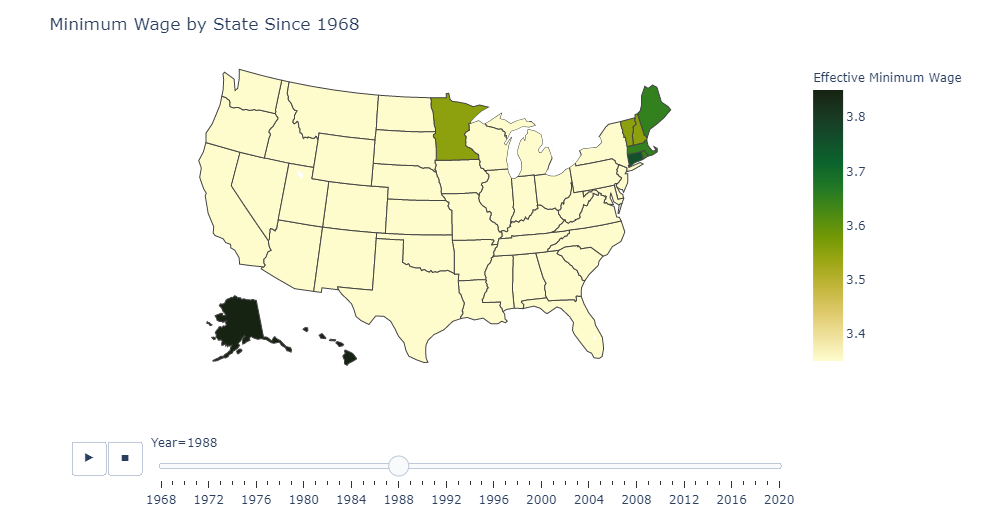
\includegraphics[width=1\textwidth]{minwage88.png}

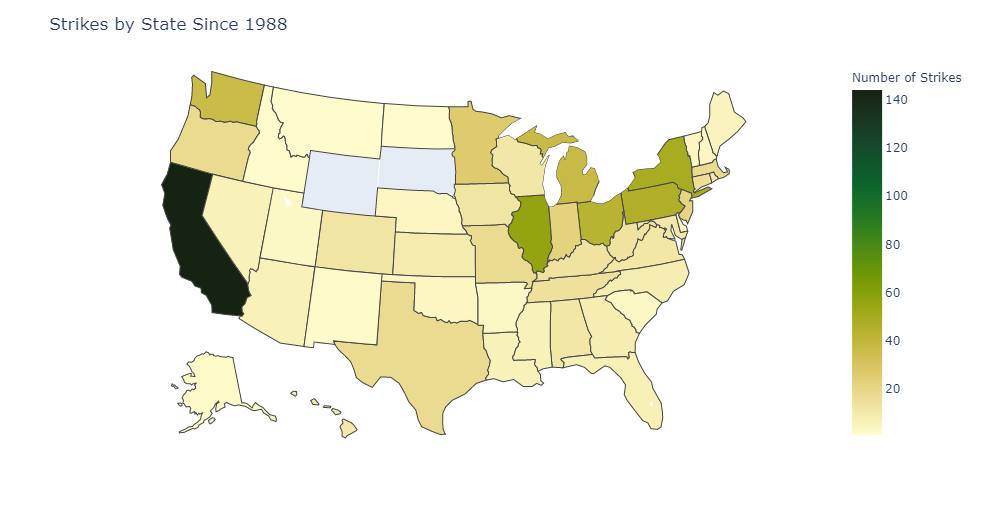
\includegraphics[width=1\textwidth]{strikes88}




Considering this statewide data, it is natural to ask exactly how do strikes distribute by state? 
For that, we have the following.

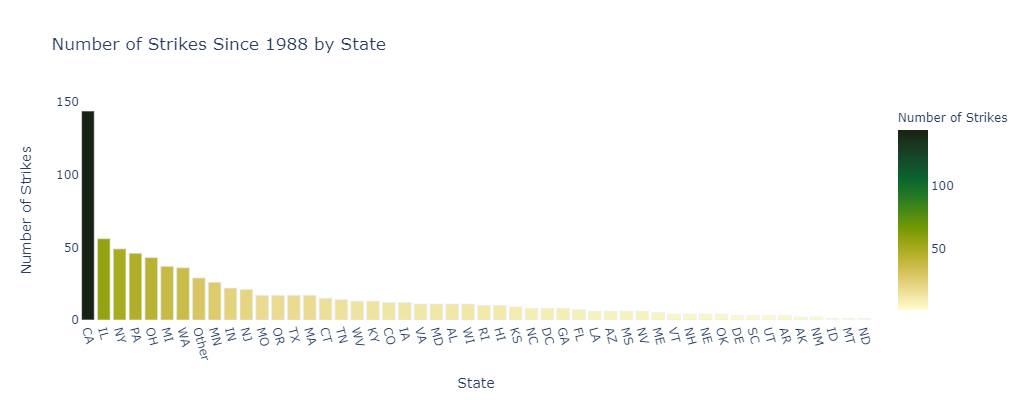
\includegraphics[width=1\textwidth]{strikesByState.png}

Given that much of our data cleaning was based around industry code, we must ask ourselves
how the strikes are distributed amongst the industries. This data is illustrated as follows.

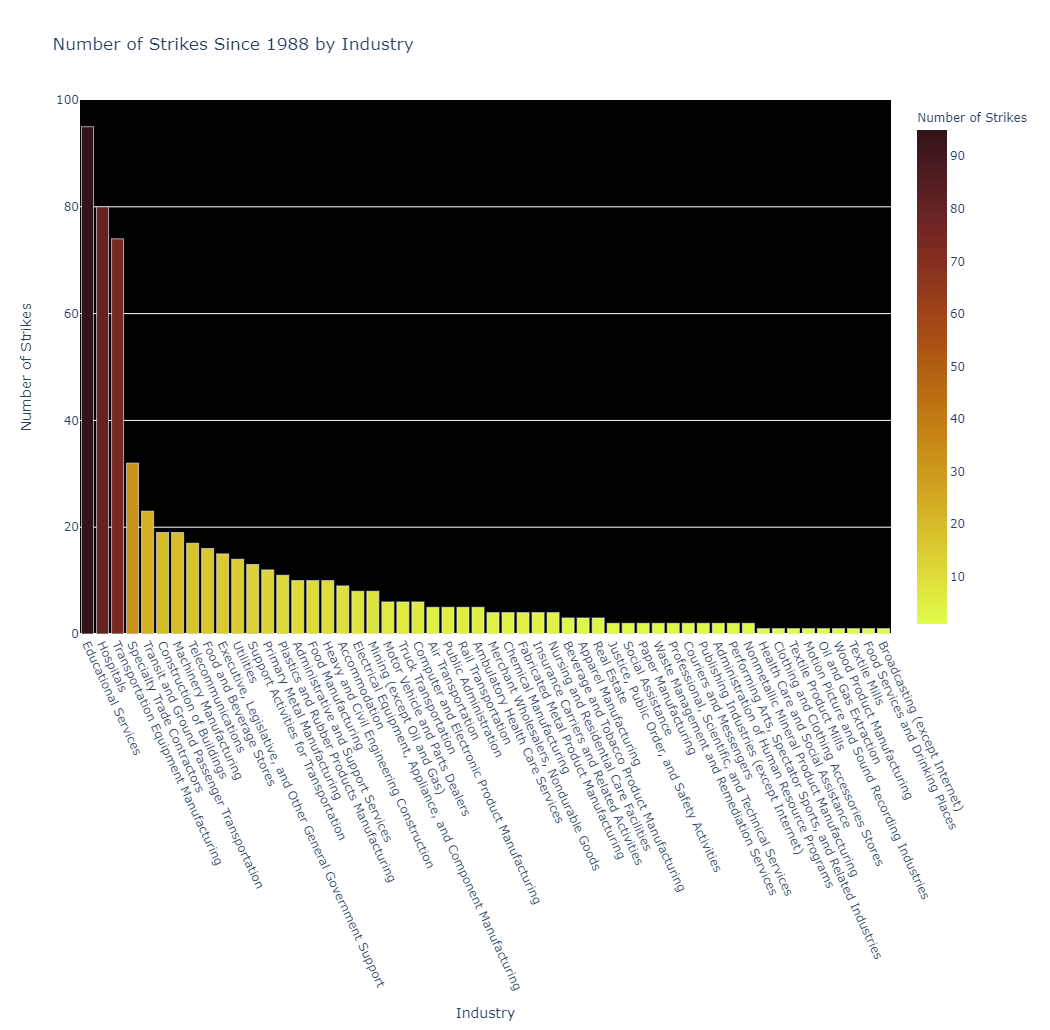
\includegraphics[width=1\textwidth]{strikesByIndustry.png}

Continuing on, what are the wages for these industries? Of course, this is provided in
the following chart.

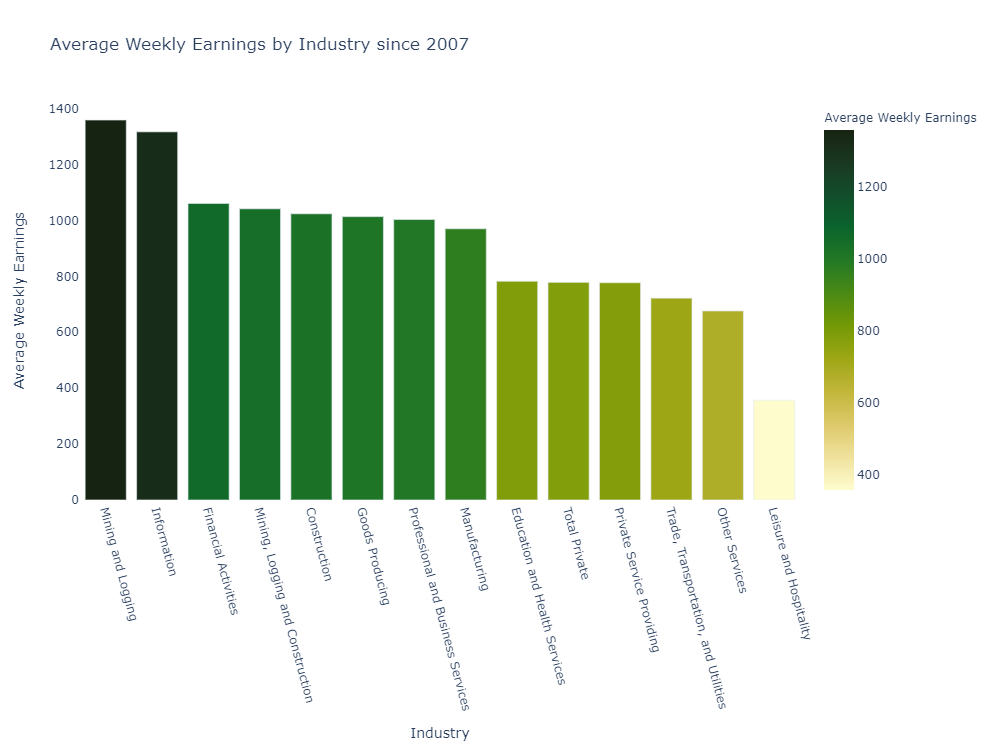
\includegraphics[width=1\textwidth]{industryWages.png}

While these are only visualizations of the data, a more detailed analysis is given in
Jupyter notebook,












\section{Conclusions}

From the visualizations of the previous section, we can see trends in the data.
We should note that this project does not follow the model of taking in data and
trying to predict future outcomes (but as noted in the literature review, this
is a common approach with strike data), but instead we are trying to analyze the
extent to which strikes still correlate to benefits to the labor force.






Unfortunately we cannot definitely drawn conclusions from this project. This is mainly due to
the problematic nature of the data. With the industry codes being improperly documented
in the the BLS data, it is unclear to what extent we are getting all the relevant data that
we want to consider. While it is true that our project shows that strikes do correlate
with increased wages, and more so than just the increase in minimum wage, we were unable 
to establish that this correlation is statistically relevant. This is not to so say
that strikes are not still a powerful tool for labor, but it is also not to say
that strikes are a powerful tool for labor. Unfortunately our conclusions were
inconclusive. Given the time, money, and man-power to truly clean and organize 
the available data, perhaps we could say otherwise.







In terms of future research, there are several obvious directions based on 
additional available data and
the 
granularity of the data. These are in line with ideas mentioned in the existing literature.
The work stoppage data includes information about the 
number of workers and the duration of the work stoppage,
so we could analyze how these numbers impact the benefits to the striking 
workers. We matched NAICS industry codes with industry codes from the 
BLS data, so we could group similar industries (both on the work stoppage side
of the data and on the BLS side) to look for patterns there.
Related to the previous two ideas, we could try to account for the
cost of that type of labor. Since we have information on the unions 
associated with the work stoppages, we could also look for patterns 
when grouping them by private versus public sector and also by
institutional versus social movement unions. 
We used data at the national and state level, there is similar data
available for metro areas (\url{https://download.bls.gov/pub/time.series/sm/})
that we could also analyze. This would require matching industry codes
similar to the state level data. Our analysis considered wage data,
but there is other relevant employment data such as 
employee injuries and illness
(\url{https://download.bls.gov/pub/time.series/cd},
\href{https://download.bls.gov/pub/time.series/cf}{CF},
\href{https://download.bls.gov/pub/time.series/ch}{CH},
\href{https://download.bls.gov/pub/time.series/fi}{FI},
\href{https://download.bls.gov/pub/time.series/fw}{FW},
\href{https://download.bls.gov/pub/time.series/hc}{HC},
\href{https://download.bls.gov/pub/time.series/hs}{HS},    
\href{https://download.bls.gov/pub/time.series/ii}{II},
\href{https://download.bls.gov/pub/time.series/sh}{SH},
\href{https://download.bls.gov/pub/time.series/si}{SI}),
employee benefits
(\href{https://download.bls.gov/pub/time.series/eb}{EB}),
unemployment and job openings
(\href{https://download.bls.gov/pub/time.series/jl}{JL},
\href{https://download.bls.gov/pub/time.series/jt}{JT},
\href{https://download.bls.gov/pub/time.series/la}{LA}),
and various costs to the employer
(\href{https://download.bls.gov/pub/time.series/cc}{CC},
\href{https://download.bls.gov/pub/time.series/ci}{CI}).
While there is a wealth of data available, each individual data set
may require us to match industry codes, which is a time consuming
process, especially since we cannot even trust the documentation of
these data sets.













\bibliographystyle{alphadin}
\bibliography{reportRef}



\end{document}